% 使用 XeLaTeX 编译；字体和图标均从项目目录加载。
\documentclass[11pt]{article}

\usepackage{fontspec}
\usepackage{xeCJK}
\usepackage{hyperref}
\usepackage{xcolor}
\usepackage{calc}
\usepackage{graphicx}
\usepackage{tikz}
\usetikzlibrary{calc}
\usepackage{enumitem}
\usepackage{titlesec}
\usepackage[
    a4paper,
    left=1.2cm,
    right=1.2cm,
    top=1.3cm,
    bottom=1.2cm,
    nohead
]{geometry}

\setmainfont[
    Path=fonts/Main/,
    Extension=.otf,
    BoldFont=texgyretermes-bold
]{texgyretermes-regular}
\setCJKmainfont[
    Path=fonts/hansans/,
    Extension=.ttf,
    BoldFont=NotoSansSC-Bold
]{NotoSansSC-Regular}
\CJKsetecglue{\hskip 0.12em}

% 兼容未安装 fontawesome 宏包的环境，复用项目附带的字体和图标定义。
\IfFileExists{fontawesome.sty}{
    \defaultfontfeatures[FontAwesome]{Path=fonts/fontawesome/opentype/}
    \usepackage{fontawesome}
}{
    \newfontfamily\FA[Path=fonts/fontawesome/opentype/]{FontAwesome.otf}
    \newcommand{\faicon}[1]{\csname faicon@##1\endcsname}
    \input{fontawesomesymbols-xeluatex.tex}
    \input{fontawesomesymbols-generic.tex}
}

\definecolor{CVBlue}{RGB}{23,110,191}
\hypersetup{
    hidelinks,
    pdftitle={蒋淇耀个人简历},
    pdfauthor={蒋淇耀}
}
\setlength{\parindent}{0pt}
\renewcommand{\baselinestretch}{1.18}
\setlist[itemize]{
    leftmargin=1.3em,
    labelsep=0.5em,
    topsep=0.25em,
    itemsep=0.12em,
    parsep=0pt,
    partopsep=0pt
}

\newlength{\interProjectSpacing}
\setlength{\interProjectSpacing}{0.45em}
\newcommand{\projectsep}{\par\vspace{\interProjectSpacing}}
\newcommand{\cvsection}[2]{%
    \section{\texorpdfstring{\makebox[1.25em][c]{\color{CVBlue}\mdseries#1}\ #2}{#2}}%
}
\titleformat{\section}
    {\large\bfseries\raggedright}{}{0em}{}
    [{\color{CVBlue}\titlerule}]
\titlespacing*{\section}{0pt}{0.7em}{0.35em}

\begin{document}
\pagenumbering{gobble}

% 保留模板的浙大标识及右上角照片；照片文件为用户提供的证件照。
\begin{tikzpicture}[remember picture,overlay]
    \node[anchor=north west,inner sep=0pt]
        at ($(current page.north west)+(0.5cm,1.0cm)$)
        {\includegraphics[height=6cm]{zju.png}};
    \node[anchor=north east,inner sep=0pt]
        at ($(current page.north east)+(-1.2cm,-0.9cm)$)
        {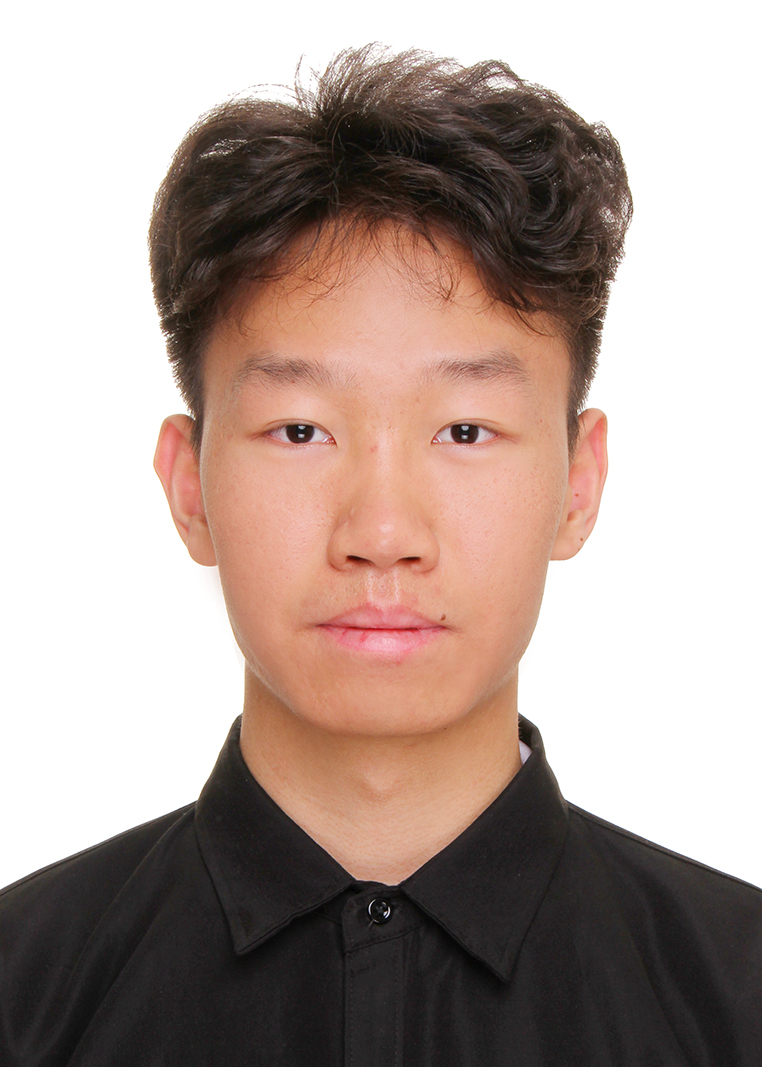
\includegraphics[height=3.4cm]{avatar.jpg}};
\end{tikzpicture}
\begin{center}
    {\LARGE\bfseries 蒋淇耀}\\[0.3em]
    {\normalsize\faEnvelopeO\ \href{mailto:3230105120@zju.edu.cn}{3230105120@zju.edu.cn}}\\[0.15em]
    {\normalsize 浙江大学\quad 预计毕业时间：2027年6月}
\end{center}
\vspace{0.1em}

\cvsection{\faGraduationCap}{教育背景}
\textbf{浙江大学\quad 数学科学学院} \hfill 2023.09 -- 2027.06（预计）\\
信息与计算科学专业\quad 理学学士\quad 浙江杭州
\begin{itemize}
    \item \textbf{学业成绩：}GPA \textbf{4.02/4.3}（88.4/100），专业排名 \textbf{10/40}。
    \item \textbf{核心课程：}数值线性代数（98）、数值分析（86）、实变函数（90）、\\
    数据结构与算法（90）、面向对象程序设计（OOP，96）、统计学习（86）。
    \item \textbf{英语水平：}大学英语六级（CET-6）：596；托福（TOEFL）：5.5（110）。
\end{itemize}

\cvsection{\faUsers}{项目与学术经历}
\textbf{高阶 B 样条插值算法实现} \hfill C++
\begin{itemize}
    \item 独立实现高阶 B 样条曲线插值算法，涵盖 2--7 阶 B 样条基函数构造、节点向量生成与导数基函数计算，支持导数边界条件、周期边界条件等多种插值条件。
    \item 采用 Cox--de Boor 递推公式计算基函数；根据插值矩阵结构，分别使用三对角矩阵 Thomas 算法和带尺度化部分选主元的 LU 分解求解线性方程组，并通过迭代改进（Iterative Refinement）提高数值稳定性。
    \item 为递归基函数求值设计记忆化缓存（Memoization），减少重复计算；设计模块化接口并完善异常处理，提高算法组件的可复用性与可维护性。
\end{itemize}

\projectsep
\textbf{数值线性代数算法库开发} \hfill C++
\begin{itemize}
    \item 独立实现 LU 分解、$LDL^{\mathsf T}$ 分解、Householder QR 分解及 QR 迭代特征值计算，构建统一的矩阵计算接口。
    \item 针对不同矩阵类型设计测试用例，比较各类分解算法在不同条件数矩阵下的数值稳定性、计算精度与效率。
\end{itemize}

\projectsep
\textbf{Math\&Control + AI 讨论班} \hfill 2026.10 -- 至今
\begin{itemize}
    \item 参与浙江大学数学科学学院组织的 Math\&Control + AI 讨论班，了解机器学习前沿内容，包括大模型训练优化算法的最新进展及大模型微调技术。
\end{itemize}

\cvsection{\faCogs}{专业技能}
\begin{itemize}
    \item \textbf{编程语言：}C++（STL），Python（NumPy、PyTorch、Pandas），MATLAB。
    \item \textbf{数学与算法：}具备扎实的数值分析、数值线性代数与泛函分析基础；熟悉矩阵分解、线性方程组求解及数值稳定性分析。
    \item \textbf{开发工具：}Git、GDB、CMake、Linux/Unix、\LaTeX。
\end{itemize}

\cvsection{\faList}{获奖情况}
\begin{itemize}
    \item 浙江大学学业优秀标兵\hfill 2023--2024、2024--2025、2025--2026 学年
    \item 浙江大学三等奖学金\hfill 2023--2024、2024--2025 学年
\end{itemize}

\end{document}
